\chapter{Evaluating the methods}
There are evidently a large variety of different methods available for solving the task at hand. Based on the work done in the previous chapter, section of the paper will discuss possible solutions to the problem. 

\section{Available data}
One important aspect that should be considered is the amount of data available for the different methods. A key criteria for the success is that there exists satellite constellations that are able to provide frequently updated image data over the requested area. New images should be available on a weekly basis, and the resolution of the images has to be approximately one meter or less for the results to be accurate enough.

\subsection*{Multispectral images}
There are many different satellite constellations that provide frequently updated multispectral imagery of the requested area, such as the Sentinel-2 \citep{ESA}, SkySat \citep{Planet2017} and WorldView \citep{DigitalGlobe2017} satellite constellations. All three constellations have a subweek revisit time over any point on earth, however the ground sampling distance (GSD) vary with a factor of more than ten.

While both SkySat and WorldView provide a submeter accuracy on their images, the Sentinel-1 constellation has a expected GSD of 10x10 meters, which will not be sufficient in terms of shadow measurement. Furthermore, it has to be taken into consideration that while data provided from the Sentinel constellations are free of charge, data from both SkySat and WorldView comes at a certain cost. Data provided by the Sentinel-2 constellation might however be accurate enough in order to locate the oil tanks. 

A general issue with multispectral images is that they are sensitive to cloudy weather and day light. This can pose as an issue if the system is expected to continuously provide data without deviations.

\subsection*{Radar images}
Another type of images that is not affected by clouds or the time of day are radar images. In terms of radar based methods, there are also a large quantity of satellite constellations that can be of interest. For example while Sentinel-2 provide multispectral images, the Sentinel-1 constellation provides radar-images with resolutions down to 5x5 meters \citep{ESA}.

WRITE MORE HERE

\section{Amount of data required for analysis}
An important difference between the different methods presented in the previous sections is the amount of data needed in order to provide an accurate analysis. For example simple image segmentation can be done in a single image using Simple Linear Iterative Clustering \citep{Achanta2012} as seen in \autoref{fig:superpixelsegmentation}. Furthermore, by knowing the approximate size of the oil tanks, a general Hough Transform \citep{Ballard1981} can be used to detect their circular shapes as seen in \autoref{fig:houghtransformcircles}. Image segmentation and shape detection using machine learning based methods require large amounts of training examples, which can be very hard to acquire. But as seen in \cite{Kaiser2017} and \cite{Kemker2017} it might be possible to automatically collect and label training data.

\begin{figure}[!h]
	\centering
	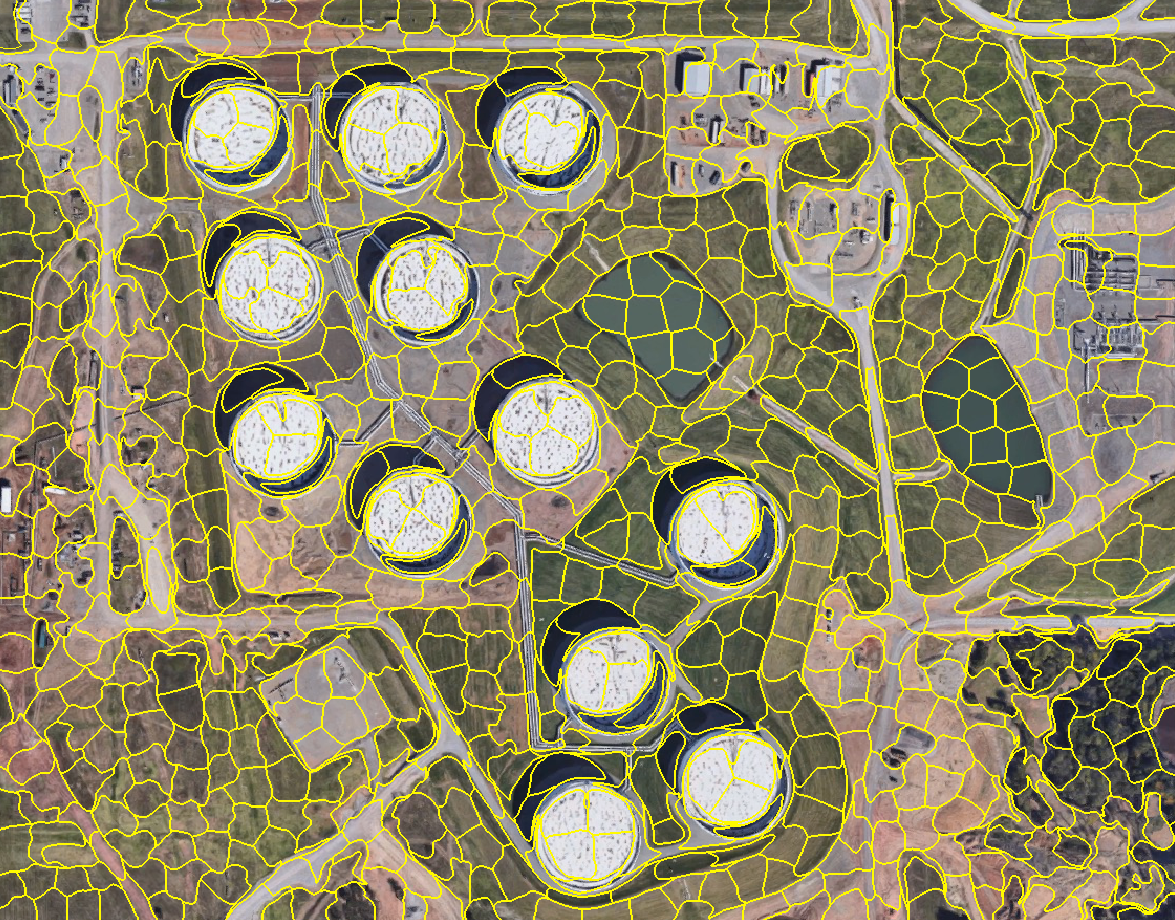
\includegraphics[scale=0.4]{fig/superpixel_segmentation.png}
	\caption{Simple implementation of SLIC superpixel segmentation on image taken from Google Earth}
	\label{fig:superpixelsegmentation}
\end{figure}

\begin{figure}[!h]
	\centering
	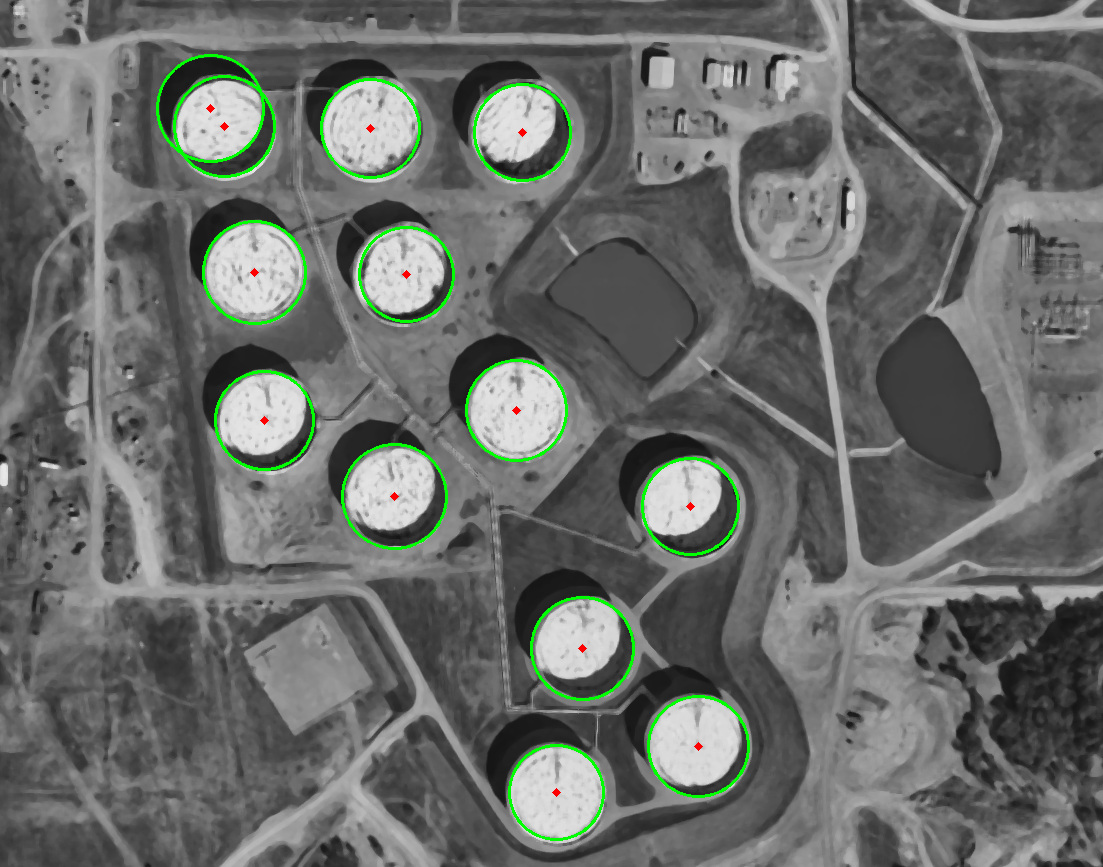
\includegraphics[scale=0.4]{fig/hough_transform_circles.png}
	\caption{Detecting circles of similar size in an image taken from Google Earth using a generalized hough transform}
	\label{fig:houghtransformcircles}
\end{figure}

Advanced methods in machine learning, such as Convolutional Neural Networks, have proven themselves as very efficient in image segmentation, but also in terms of classifying the different segments and even associating values with them if given the correct training data. This means that by acquiring the correct training data, which in this setting would be the the actual inventory of an oil tank at a certain time, and relate these values to aerial photographs of the same tanks, it would be possible to train a network into doing the actual inventory estimation directly.

When it comes to height estimation using radar images, \cite{Brunner2008} presented a method that only acquired a single radar image in order to estimate the height of buildings using the SAR principle. In order to generate a interferogram two phase images are required as explained in \cite{Liu2015}. Furthermore, height estimation using shadow measurement can also be done using single, multispectral images as shown by \cite{Comber2012} and \cite{Shao2011}.

\section{Choosing a method}
By taking the above comparison into consideration, it becomes clear that in terms of pure circle detection, the generalized Hough transform stands out as the most efficient method. The fact that we have pre-knowledge about the shape of the objects we are trying to locate, makes it much easier to use a standard approach. However, the generalized Hough transform isolated will not be able to estimate any heights, and would have to be combined with another method for height estimation. By looking at \autoref{fig:houghtransformcircles}, height estimation using shadow measurements might be the best approach. This is because the green circles limits the search area in terms of locating shadows, since we are only interested in the shadow that is cast inside the tanks.

An important issue regarding the generalized hough transform is the fact that if the tanks vary in size, it might not be able to find all of them, as seen in \autoref{fig:houghtransformdifference}.

\begin{figure}[!h]
	\centering
	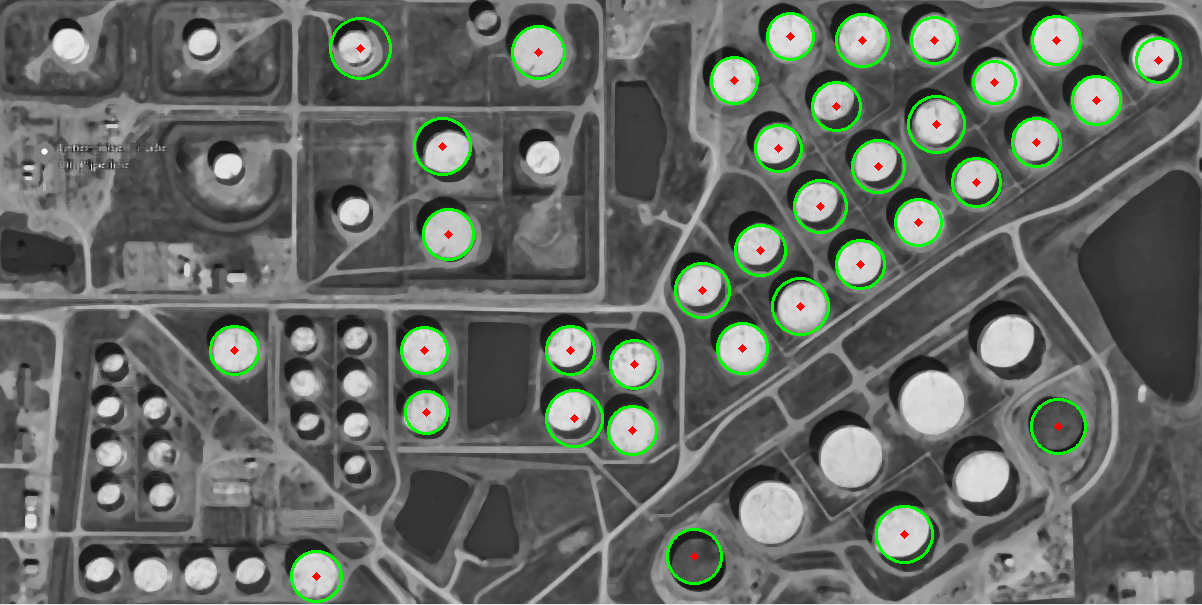
\includegraphics[scale=0.35]{fig/hough_transform_difference.png}
	\caption{Detecting circles of different size in an image taken from Google Earth using a generalized hough transform}
	\label{fig:houghtransformdifference}
\end{figure}

Looking at \autoref{fig:superpixelsegmentation} it seems like the SLIC algorithm has potential in terms of image segmentation as well, but an issue is that it is hard to extract the correct edges without any prior knowledge. And the same issue regarding height estimation arises, since the algorithm will have to be combined with another method.

As previously stated, it has been shown that convolutional neural networks outperform the state-of-the-art methods for image segmentation in terms of accuracy, if they are provided with enough good training examples. There are several ways of acquire training data, such as automatically extract training examples from OpenStreetMap as described by \cite{Kaiser2017}. 

Since 2012 convolutional networks have been the leading method for object recognition and image segmentation. Furthermore, very deep convolutional neural networks such as the ResNet \citep{Wu2017} have shown an incredible ability to create very complex functions for image analysis. The potential of these networks have yet not been fully explored, and there are still many applications that have not been discovered. One of them being building height extraction from aerial imagery.

After comparing the different methods, it has become clear that there are many ways to attack the presented problem. Below x different methods are presented as potential approaches to solving the problem:

\begin{itemize}
    \item Direct estimation of the tanks inventory from shadow measurements using a modified ResNet
    \item Using a generalized Hough transform for tank detection, thus limiting the shadow search space, and then applying a modified ResNet for estimating a single tanks inventory.
\end{itemize}